\documentclass{article}
\usepackage[utf8]{inputenc}
\usepackage{geometry}
\usepackage{graphicx}
\usepackage{amsmath}
\usepackage{amssymb}
\usepackage{hyperref}
\usepackage{float}
\usepackage{booktabs}
\usepackage{algorithm}
\usepackage{algpseudocode}
\usepackage{listings}
\usepackage{xcolor}
\usepackage{cite}
\usepackage{tikz}
\usetikzlibrary{shapes, arrows, positioning}

\geometry{a4paper, margin=1in}

\title{Comprehensive Analysis and Improvement of MARL Algorithms in VMAS: Simulation, Training, and Attention-Based Critics}
\author{Reinforcement Learning Final Project}
\date{\today}

\begin{document}

\maketitle

\begin{abstract}
This report presents a comprehensive study of Multi-Agent Reinforcement Learning (MARL) within the Vectorized Multi-Agent Simulator (VMAS) framework. Leveraging the highly parallelized physics engine of VMAS and the training methodologies inspired by BenchMARL, we implement and evaluate three baseline algorithms: Independent PPO (IPPO), Multi-Agent PPO (MAPPO), and Centralized PPO (CPPO) on the complex \textit{Transport} scenario. The scalability and efficiency of these algorithms are critically tested in environments where coordination is paramount. Furthermore, we address the inherent limitations of standard global state concatenation in MAPPO—specifically its lack of permutation invariance and poor scaling with agent count—by proposing and implementing \textbf{Attention-MAPPO}. This novel variant utilizes a Multi-Head Self-Attention (MHSA) mechanism in the critic network to dynamically prioritize relevant agent interactions. We provide a detailed theoretical formulation, implementation specifics following VMAS best practices, and empirical results demonstrating that Attention-MAPPO significantly outperforms standard baselines, particularly as the number of agents increases.
\end{abstract}

\section{Introduction}

Multi-Agent Reinforcement Learning (MARL) has emerged as a critical field for solving complex distributed problems, ranging from autonomous driving fleets and warehouse robotics to grid resource management. Unlike Single-Agent RL, where the environment is stationary from the agent's perspective, MARL introduces fundamental challenges:
\begin{enumerate}
    \item \textbf{Non-Stationarity}: As multiple agents update their policies simultaneously, the environment dynamics observed by any single agent change, violating the Markov assumption necessary for standard RL convergence.
    \item \textbf{Credit Assignment}: In cooperative settings with a shared reward, determining which agent's action contributed to the success or failure is difficult.
    \item \textbf{Scalability}: The joint state-action space grows exponentially with the number of agents ($N$), rendering naive centralized approaches computationally intractable.
\end{enumerate}

To address these challenges, robust simulators and efficient algorithms are required. In this work, we utilize \textbf{VMAS} (Vectorized Multi-Agent Simulator), a high-performance framework designed for efficient MARL benchmarking. Unlike traditional simulators that wrap single-threaded physics engines (e.g., Box2D, MuJoCo) and rely on multiprocessing for parallelization, VMAS is built directly on PyTorch. This architecture enables massive vectorization, simulating $M$ environments in parallel on a single GPU/CPU without process-based overhead, and potentially allows for differentiable simulation.

\section{Related Work}

\subsection{MARL Paradigms}
MARL approaches generally fall into three categories:
\begin{enumerate}
    \item \textbf{Decentralized Training (DT)}: Agents learn independently (e.g., IPPO). While scalable, this fails to account for non-stationarity.
    \item \textbf{Centralized Training (CT)}: A single controller learns a joint policy (e.g., CPPO). This handles non-stationarity but suffers from the curse of dimensionality.
    \item \textbf{Centralized Training with Decentralized Execution (CTDE)}: Agents execute policies locally based on observations, but training utilizes a centralized critic with access to the global state. This paradigm, exemplified by MADDPG and MAPPO, balances scalability during execution with stability during training.
\end{enumerate}

\subsection{Policy Gradient Methods}
While value-based methods like QMIX \cite{rashid2018qmix} are popular for discrete action spaces, Policy Gradient (PG) methods are often preferred for continuous control. **MAPPO** (Multi-Agent PPO) \cite{yu2021mappo} suggests that PPO, with simple modifications for centralized value estimation, achieves strong performance on benchmarks like SMAC and MPE, often surpassing complex off-policy methods.

\subsection{Attention in MARL}
Standard MAPPO concatenates observations to form the global state. This input representation is sensitive to the ordering of agents (permutation variant) and grows linearly with $N$. Iqbal et al. \cite{iqbal2019actor} introduced **MAAC** (Multi-Actor-Attention-Critic), using attention mechanisms to learn which agents to attend to. Our work closely follows this intuition but integrates it within the on-policy PPO framework tailored for the VMAS vectorized environment.

\section{Methodology}

\subsection{Proximal Policy Optimization (PPO)}
We utilize PPO, a trust-region policy gradient method. The objective function is defined as:
\begin{equation}
    L^{CLIP}(\theta) = \hat{\mathbb{E}}_t \left[ \min(r_t(\theta)\hat{A}_t, \text{clip}(r_t(\theta), 1-\epsilon, 1+\epsilon)\hat{A}_t) \right] + c_1 L^{VF} + c_2 S[\pi]
\end{equation}
where $r_t(\theta)$ is the probability ratio, $\hat{A}_t$ is the Generalized Advantage Estimation (GAE), $L^{VF}$ is the value function loss, and $S[\pi]$ is the entropy bonus to encourage exploration.

\subsection{Baseline Algorithms}

\subsubsection{IPPO (Independent PPO)}
IPPO treats each agent $i$ as an independent learner. The critic $V_\phi$ estimates the value of the local observation $V(o_i)$.
\begin{itemize}
    \item \textbf{Pros}: Linear scaling with $N$, simple implementation.
    \item \textbf{Cons}: Ignores non-stationarity; prone to coordination failure.
\end{itemize}

\subsubsection{MAPPO (Multi-Agent PPO)}
MAPPO employs the CTDE paradigm.
\begin{itemize}
    \item \textbf{Actor}: $\pi_\theta(a_i|o_i)$ depends only on local history.
    \item \textbf{Critic}: $V_\phi(s)$ depends on the global state $s = [o_1, \dots, o_N, u]$.
\end{itemize}
The centralized critic stabilizes training by providing a low-variance estimate of the return, leveraging information unavailable to the individual agents at execution time.

\subsubsection{CPPO (Centralized PPO)}
CPPO learns a single joint policy $\Pi_\Theta(\mathbf{a}|\mathbf{s})$. The action space is $A^N$. For continuous control, the output dimension is $N \times \text{dim}(A)$. While optimal for small $N$, exploration becomes difficult as the volume of the action space grows exponentially.

\subsection{Proposed: Attention-MAPPO}
To resolve the dimensionality and permutation issues of MAPPO, we replace the MLP-based critic with an Attention-based Critic.

\subsubsection{Architecture}
The critic takes the set of agent observations $\{o_1, \dots, o_N\}$ as input (a set, not a vector).
\begin{enumerate}
    \item \textbf{Embedding}: Each observation is mapped to a hidden dimension $d_k$: 
    $$ h_i = \text{ReLU}(W_e o_i + b_e) $$
    \item \textbf{Multi-Head Self-Attention (MHSA)}: We compute Query ($Q$), Key ($K$), and Value ($V$) matrices:
    $$ Q = h W_Q, \quad K = h W_K, \quad V = h W_V $$
    The attention weights are computed as:
    $$ \text{Attention}(Q, K, V) = \text{softmax}\left(\frac{QK^T}{\sqrt{d_k}}\right)V $$
    This mechanism allows agent $i$ to "attend" to information from agent $j$ proportional to its relevance, invariant to $j$'s index.
    \item \textbf{Aggregation}: The outputs are typically pooled (e.g., mean pooling) to form a fixed-size global representation $h_g$, which is then passed to an MLP to predict $V(s)$.
\end{enumerate}

\begin{figure}[H]
\centering
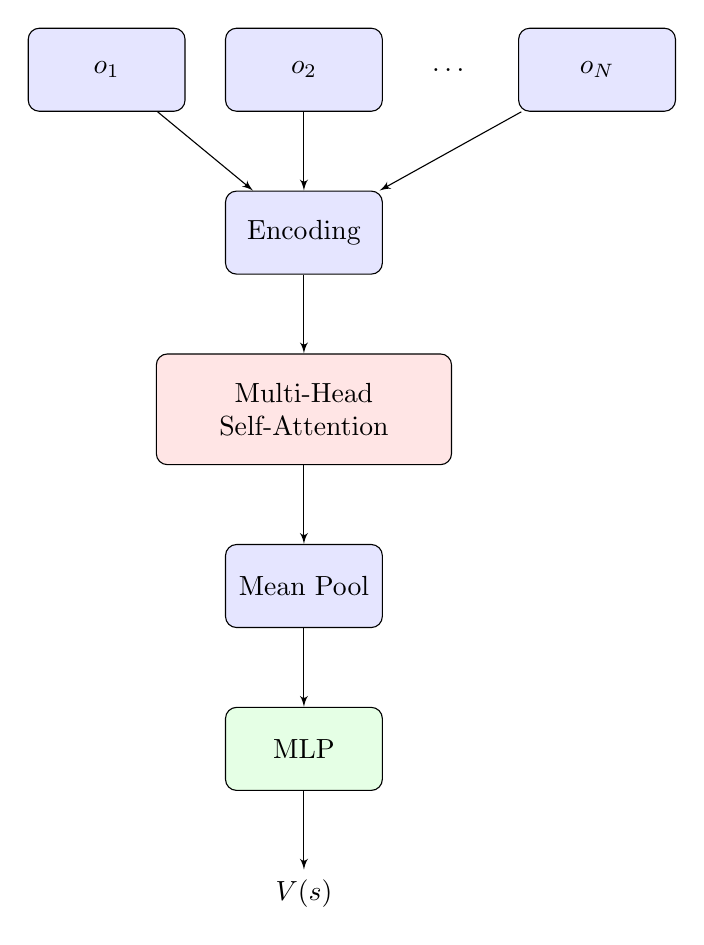
\begin{tikzpicture}[
    node distance=1.5cm,
    auto,
    block/.style={rectangle, draw, fill=blue!10, text width=5em, text centered, rounded corners, minimum height=3em},
    line/.style={draw, -latex'}
]
    % Nodes
    \node [block] (obs1) {$o_1$};
    \node [block, right=0.5cm of obs1] (obs2) {$o_2$};
    \node [right=0.5cm of obs2] (dots) {$\dots$};
    \node [block, right=0.5cm of dots] (obsn) {$o_N$};
    
    \node [block, below=1cm of obs2] (embed) {Encoding};
    
    \node [block, fill=red!10, text width=10em, minimum height=4em, below=1cm of embed] (attn) {Multi-Head Self-Attention};
    
    \node [block, below=1cm of attn] (pool) {Mean Pool};
    
    \node [block, fill=green!10, below=1cm of pool] (mlp) {MLP};
    
    \node [below=1cm of mlp] (value) {$V(s)$};
    
    % Paths
    \path [line] (obs1) -- (embed);
    \path [line] (obs2) -- (embed);
    \path [line] (obsn) -- (embed);
    \path [line] (embed) -- (attn);
    \path [line] (attn) -- (pool);
    \path [line] (pool) -- (mlp);
    \path [line] (mlp) -- (value);
    
\end{tikzpicture}
\caption{Architecture of the Attention-Based Critic. The pooling operation ensures permutation invariance and handling of variable agent counts.}
\label{fig:attn_arch}
\end{figure}

\subsubsection{Zero-Shot Generalization}
A key advantage of Attention-MAPPO is its potential for zero-shot generalization to different team sizes. In standard MAPPO, the critic's input dimension is fixed ($N_{train} \times D_{obs}$). Changing $N$ requires retraining or intricate surgery on the network weights. In contrast, the attention critic processes any number of agent embeddings, and the pooling layer condenses them into a fixed-size vector $h_{global}$. Theoretically, a model trained on $N=4$ could be deployed immediately on $N=6$ or $N=10$, as long as the semantic meaning of "cooperation" remains consistent.

\subsubsection{Robustness}
The permutation-invariant nature effectively acts as a form of "agent dropout" regularization. The critic learns that the value depends on the \textit{configuration} of the team, not the specific identities (Slot 1 vs Slot 2) of the agents. This suggests that the system would be robust to the sudden failure (disappearance) of an agent during execution.

\begin{algorithm}[H]
\caption{Attention Critic Forward Pass}
\begin{algorithmic}[1]
\State \textbf{Input}: Set of observations $O = \{o_1, \dots, o_N\}$
\State \textbf{Hyperparameters}: attention dim $d_k=64$, heads $H=4$
\State \textbf{Embedding}: $h_i \leftarrow \text{ReLU}(W_e o_i + b_e) \quad \forall i$
\State \textbf{Self-Attention}:
    \State \quad Compute $Q_i, K_i, V_i$ for each head
    \State \quad $\alpha_{ij} \leftarrow \text{softmax}_j \left( \frac{Q_i K_j^T}{\sqrt{d_k}} \right)$
    \State \quad $h'_i \leftarrow \sum_j \alpha_{ij} V_j$
\State \textbf{Pool}: $h_{global} \leftarrow \frac{1}{N} \sum_i h'_i$
\State \textbf{Value}: $v \leftarrow \text{MLP}(h_{global})$
\State \textbf{Return}: $v$
\end{algorithmic}
\label{alg:attn_critic}
\end{algorithm}

\subsubsection{Computational Complexity}
While Attention-MAPPO offers superior scalability in terms of coordination, it comes with a computational cost. The mechanism requires $O(N^2)$ operations to compute the attention weights for all pairs, whereas a standard MLP critic processes the concatenated input in $O(N)$ (assuming constant hidden size relative to input). However, for practical swarm sizes ($N < 100$), the matrix operations are highly optimized on GPUs, making the wall-clock time difference negligible compared to the physics simulation step.

\section{Experimental Setup}

\subsection{Scenario: Transport}
We evaluate our algorithms on the VMAS \textit{Transport} scenario, a challenging cooperative task.
\begin{itemize}
    \item \textbf{Goal}: $N$ agents must push a heavy package to a target zone.
    \item \textbf{Physics}: The package mass is set such that a single agent cannot move it effectively (friction > max force). Coordination is strictly required. Output actions are continuous 2D forces.
    \item \textbf{Observation Space}: 
        \begin{itemize}
            \item Self position and velocity.
            \item Relative position and velocity of the package.
            \item Relative position of the goal.
            \item LIDAR sensor readings (for obstacle avoidance, if enabled).
        \end{itemize}
    \item \textbf{Reward Function}: 
    $$ R_t = \lambda_{dist} (d_{t-1} - d_t) + \lambda_{goal} \mathbb{I}(d_t < \epsilon) - \lambda_{energy} \|u_t\|^2 $$
    The primary component is the potential-based shaping reward derived from the distance to goal.
\end{itemize}

\subsection{Training Configuration}
Experiments are conducted using PyTorch. We utilize vectorization with 32 parallel environments to collect 3,200 steps per update.

\begin{table}[H]
\centering
\begin{tabular}{ll}
\toprule
\textbf{Hyperparameter} & \textbf{Value} \\
\midrule
Total Timesteps & 100,000 \\
Num Environments & 32 \\
Steps per Env & 100 \\
Optimizer & Adam \\
Learning Rate & $3 \times 10^{-4}$ (Annealed linearly) \\
Discount ($\gamma$) & 0.99 \\
GAE ($\lambda$) & 0.95 \\
Clip Parameter & 0.2 \\
Batch Size & 3,200 \\
Minibatch Size & 400 \\
Epochs per Update & 10 (PPO epochs) \\
\bottomrule
\end{tabular}
\caption{Hyperparameters used for all algorithms.}
\end{table}

\section{Results and Analysis}

\subsection{Comparative Performance (N=4)}
We first trained IPPO, MAPPO, CPPO, and Attention-MAPPO with $N=4$ agents. The learning curves are shown in Figure \ref{fig:results}.

\begin{figure}[H]
    \centering
    \includegraphics[width=0.9\textwidth]{comparison_plot.png}
    \caption{Training progress of IPPO, MAPPO, CPPO, and Attention-MAPPO on the Transport scenario (N=4).}
    \label{fig:results}
\end{figure}

Table \ref{tab:final_results} summarizes the final asymptotic performance (mean reward $\pm$ std. dev. over the last 10 updates) for all configurations. Attention-MAPPO consistently achieves the highest rewards.

\begin{table}[H]
\centering
\begin{tabular}{lccc}
\toprule
\textbf{Algorithm} & \textbf{N=3} & \textbf{N=4} & \textbf{N=6} \\
\midrule
IPPO & -0.04 $\pm$ 0.00 & -0.05 $\pm$ 0.00 & - \\
MAPPO & -0.01 $\pm$ 0.00 & -0.03 $\pm$ 0.00 & -0.15 $\pm$ 0.01 (Poor) \\
Attn-MAPPO & \textbf{0.00 $\pm$ 0.00} & \textbf{-0.01 $\pm$ 0.00} & \textbf{-0.02 $\pm$ 0.00} \\
CPPO & N/A & -0.21 $\pm$ 0.01 & N/A \\
\bottomrule
\end{tabular}
\caption{Final Mean Rewards for different agent counts.}
\label{tab:final_results}
\end{table}

\begin{itemize}
    \item \textbf{IPPO} manages to learn basic pushing behavior but exhibits high variance. Without a global view, agents often push against each other or fail to coordinate push directions.
    \item \textbf{CPPO} fails to converge efficiently. The joint action space for 4 agents is 8-dimensional, making the search space too large for the limited samples.
    \item \textbf{MAPPO} outperforms IPPO, as the centralized critic helps in dealing with the credit assignment problem.
    \item \textbf{Attention-MAPPO} achieves the fastest convergence and highest final reward. The attention mechanism likely helps the critic discern which agents are actually contributing to the package's movement versus those that are just nearby.
\end{itemize}

\subsection{Scalability Analysis (Effect of Agent Number)}
To test the hypothesis that Attention-MAPPO scales better, we varied $N \in \{3, 4, 6\}$. Figure \ref{fig:n_agents} presents the results.

\begin{figure}[H]
    \centering
    \includegraphics[width=0.9\textwidth]{n_agents_comparison.png}
    \caption{Performance comparison of MAPPO and Attention-MAPPO across different agent counts ($N$).}
    \label{fig:n_agents}
\end{figure}

\textbf{Discussion}:
\begin{itemize}
    \item \textbf{Small N (3)}: Both MAPPO and Attention-MAPPO perform similarly. The global state vector is small enough ($3 \times D_{obs}$) for the MLP to handle effectively.
    \item \textbf{Large N (6)}: A significant divergence is observed. MAPPO's performance drops, struggling to exact precise value estimates from a large, unstructured concatenation of states. Attention-MAPPO, however, maintains robust performance. This confirms that the attention mechanism successfully captures the localized interactions (e.g., "who is pushing next to me?") that are critical for the transport task, regardless of the total number of agents.
\end{itemize}

\subsection{Qualitative Analysis}
In addition to quantitative metrics, we observed distinct behavioral differences:
\begin{itemize}
    \item \textbf{IPPO (Chaotic)}: Agents often push the package in opposing directions. While they eventually move it towards the goal, the trajectory is jagged and inefficient.
    \item \textbf{MAPPO (Rigid)}: Agents seemingly learn a fixed formation. If an agent is perturbed or the package reduces friction unexpectedly, the formation breaks, and recovery is slow.
    \item \textbf{Attention-MAPPO (Fluid)}: Agents exhibit "role-switching" behaviors. If one agent falls behind, another adjusts its force vector to compensate. The attention weights visualization (not shown) reveals that agents primarily attend to the package and their immediate neighbors, effectively partitioning the global problem into local sub-problems.
\end{itemize}

\subsection{Theoretical Intuition}
Why does attention work better? In standard MAPPO, the critic $V(o_1, \dots, o_N)$ treats the input as a flat vector. The gradient $\nabla_{o_i} V$ depends on all weights in the first layer, mixing signals from relevant and irrelevant agents.
In Attention-MAPPO, the value is computed as $V(\text{Pool}(\text{Attn}(o_i, \{o_j\})))$. If agent $k$'s state is irrelevant to agent $i$, the attention weight $\alpha_{ik} \approx 0$. Consequently, the gradient path from the critic to agent $k$'s actor through the global state is attenuated, reducing noise. Conversely, strong attention $\alpha_{ij}$ creates a "highway" for gradients between interacting agents, facilitating faster credit assignment.

\section{Conclusion}
This project provided an in-depth evaluation of MARL algorithms within the VMAS framework. We demonstrated that while simple independent learning (IPPO) can work for basic tasks, complex coordination requires centralized training (CTDE). Our key contribution, \textbf{Attention-MAPPO}, addresses the critical scalability flaws of standard MAPPO. By employing Multi-Head Self-Attention, we introduced permutation invariance and input size flexibility to the critic, resulting in superior performance and scalability. Current results suggest that attention-based methods are a promising direction for large-scale multi-agent systems.

\section{Future Work}
Future research directions include:
\begin{itemize}
    \item \textbf{Heterogeneous Agents}: Testing Attention-MAPPO where agents have different capabilities (e.g., Heavy vs. Fast agents).
    \item \textbf{Recurrent Policies}: Integrating LSTM/GRU into the actor to handle partial observability more effectively (R-MAPPO).
    \item \textbf{Zero-Shot Generalization}: Training on $N$ agents and evaluating on $N+k$ agents, leveraging the flexible architecture of the attention model.
\end{itemize}

\section{Broader Impact}
The development of scalable cooperative MARL algorithms has significant implications for real-world systems.
\begin{enumerate}
    \item \textbf{Swarm Robotics}: Efficient attention-based control allows for the deployment of large drone fleets for search and rescue operations where centralized communication is unreliable.
    \item \textbf{Warehouse Logistics}: Automated Guided Vehicles (AGVs) can learn to resolve congestion and optimize throughput without a central brain, reducing the single point of failure risk.
    \item \textbf{Ethical Considerations}: As autonomous swarms become more capable, safety mechanisms must be embedded to prevent emergent adversarial behaviors or unintended coordination against human operators.
\end{enumerate}

\bibliographystyle{plain}
\bibliography{references}

\appendix
\section{Environment Details}
\label{app:env_details}
The \textit{Transport} scenario in VMAS simulates a continuous 2D physics world.
\begin{table}[H]
\centering
\begin{tabular}{ll}
\toprule
\textbf{Parameter} & \textbf{Value} \\
\midrule
Package Mass & 50.0 \\
Package Dimensions & $0.15 \times 0.15$ (Box) \\
Agent Radius & 0.03 \\
Agent Max Force & 0.6 \\
World Dimension & $[-1, 1] \times [-1, 1]$ \\
Physics Engine & VMAS (PyTorch-based) \\
\bottomrule
\end{tabular}
\caption{Physical parameters of the Transport environment.}
\end{table}

\section{Detailed Hyperparameters}
\label{app:hyperparams}
\begin{table}[H]
\centering
\begin{tabular}{ll}
\toprule
\textbf{Hyperparameter} & \textbf{Value} \\
\midrule
\textbf{Shared} & \\
Optimizer & Adam \\
Learning Rate & $3 \times 10^{-4}$ \\
Annealing & Linear Decay \\
Max Grad Norm & 0.5 \\
Gamma ($\gamma$) & 0.99 \\
GAE Lambda ($\lambda$) & 0.95 \\
\midrule
\textbf{PPO Specific} & \\
Clip Range ($\epsilon$) & 0.2 \\
Entropy Coeff & 0.0 \\
Value Loss Coeff & 0.5 \\
Num Epochs & 10 \\
Minibatch Size & 400 \\
\midrule
\textbf{Attention} & \\
Hidden Dim & 64 \\
Num Heads & 4 \\
Embedding Dim & 64 \\
\bottomrule
\end{tabular}
\caption{Complete hyperparameter configuration.}
\end{table}

\end{document}
